%
%  $Description: A Haskell Interpreter for Object Calculus
%

\documentclass[10pt,twocolumn]{article}
\usepackage{times,mathptmx,fullpage}
% Allows you to put literal text into your document without having
% LaTeX try to interpret it.
\usepackage{verbatim}
% Sorts citations numerically and "combines" adjacent ones
\usepackage{cite}
% Allows you to individually label subfigures in a multi-part figure
\usepackage{subfigure}
% Allows the definition of macros that are smart about adding space
% after text in a macro
\usepackage{xspace}
\usepackage{graphicx}
\graphicspath{/}

% Redefine the percentage of the page that can be used for floats (figures,
% tables, etc.)
\renewcommand\floatpagefraction{.9}
\renewcommand\dblfloatpagefraction{.9}
\renewcommand\topfraction{.9}
\renewcommand\dbltopfraction{.9}
\renewcommand\bottomfraction{.9}
\renewcommand\textfraction{.1}
\setcounter{totalnumber}{10}
\setcounter{topnumber}{10}
\setcounter{dbltopnumber}{10}
\setcounter{bottomnumber}{10}

% Code Snippets
\usepackage{listings}
\usepackage{color}

\definecolor{dkgreen}{rgb}{0,0.6,0}
\definecolor{gray}{rgb}{0.5,0.5,0.5}
\definecolor{mauve}{rgb}{0.58,0,0.82}

\lstset{frame=tb,
  language=Haskell,
  aboveskip=3mm,
  belowskip=3mm,
  showstringspaces=false,
  columns=flexible,
  basicstyle={\small\ttfamily},
  numbers=none,
  numberstyle=\tiny\color{gray},
  keywordstyle=\color{blue},
  commentstyle=\color{dkgreen},
  stringstyle=\color{mauve},
  breaklines=true,
  breakatwhitespace=true,
  tabsize=3
}


% Set values for float separation from text
\setlength{\floatsep}{1.5ex plus1.0ex minus 0.2ex}
\setlength{\dblfloatsep}{1.5ex plus1.0ex minus 0.2ex}
\setlength{\textfloatsep}{1.5ex plus1.0ex minus 0.2ex}
\setlength{\dbltextfloatsep}{1.5ex plus1.0ex minus 0.2ex}
\setlength{\abovecaptionskip}{0.5ex}
\setlength{\belowcaptionskip}{0.5ex}

% Don't allow widows or clubs - single lines at the start/end of a column
\widowpenalty=10000
\clubpenalty=10000

\newcommand{\latex}{\LaTeX\xspace}
\pagestyle{plain}

%------------------------------------------------------------------------- 
\begin{document}

\title{A Haskell Interpreter for Object Calculus}

\author{
Shobhit Maheshwari \\
\textit{Univ. of California, Santa Cruz} \\
\textit{shmahesh@ucsc.edu}
\and
Aneesh Neelam \\
\textit{Univ. of California, Santa Cruz} \\
\textit{aneelam@ucsc.edu}
}

\maketitle
\thispagestyle{empty}

\begin{abstract}
We present an interpreter developed in Haskell for the Object Calculi introduced and detailed by M. Abadi and L. Cardelli.  Object Calculus has been devised to represent objects directly as primitives, rather than to try to make use of Lambda Calculus that use function primitives, to objects. Since Haskell is not an object oriented language, we shall be deviating slightly from the syntax of the Object Calculi in our interpreter. But the Haskell interpreter will be based on the semantics, and typing rules of object-oriented languages specified by these Object Calculi. 
\end{abstract}

%------------------------------------------------------------------------- 
\section{Introduction}

Lambda Calculus has been introduced by Church in the 1930s as a formal system in mathematical logic to express computation based on function abstraction and application using variable binding and substitution \cite{ex3, ex7}. Church numerals and encoding are used to represent data and operators in Lambda Calculus \cite{ex4}. Functions are primitives in Lambda Calculus, and are directly implemented by functional programming languages. 

For a given Lambda Calculus, one can implement a Haskell interpreter trivially. Various Lambda Calculi have been used as a foundation for procedural languages \cite{ex11}. Interpreters can be built quickly for them. 

However, Object-Oriented languages cannot be represented easily by Lambda Calculus. Object Oriented Programming constructs like Inheritance, Polymorphism cannot be represented easily by the Lambda Calculus and notation devised by Church. This is especially true for typed Object Oriented languages, when using typed Lambda Calculus \cite{ex1}. It is not trivial even with Object Calculus to develop an interpreter in Haskell, a typed functional language, but it certainly is easier than directly adapting Lambda Calculus for object-oriented languages and then developing an interpreter for that \cite{ex11}. 

Abadi and Cardelli devised Object Calculus to complement Lambda Calculus, and help represent object-oriented concepts in programming languages more easily \cite{ex1,ex2,ex6,ex11}. There are a number of approaches that others have tried with various degrees of success when representing these languages and concepts. 

In the next section, we shall see approaches that others have taken to model object-oriented languages, either adapting or directly using Lambda Calculus or in this case, devising a new formal mathematical system. In Section III, we shall have a quick overview of the Object Calculi devised by Abadi and Cardelli \cite{ex11}, and walk through the given syntax. In Section IV, we shall present our Haskell interpreter for untyped imperative Object Calculi, and in Section V, we conclude and discuss future work. 

%------------------------------------------------------------------------- 
\section{Related Work}

These are the broad approaches taken to model object-oriented languages. More work has been done pertaining to each of the following approaches. 

One of the earliest approaches to developing a formal system for modeling object-oriented languages was to use typed Lambda Calculus to encode objects, classes and methods in more primitive constructs like functions. Pierce specifies how lambdas and recursive records can be used to obtain a foundation for object oriented languages \cite{ex8}. However, Abadi and Cardelli argue that Lambda Calculus is quite unsuitable for representing some of the concepts in object-oriented languages and hence devised Object Calculus \cite{ex1, ex11}. 

Castagna uses multimethod calculus to help represent object oriented theory and abstractions \cite{ex9}. This approach is somewhat similar to Object Calculus, but it is more verbose and complicated. Object Calculus was devised to have a minimal syntax \cite{ex11}. 

Bruce devised class-based calculi to model class-based programming. But the focus is on class-based languages, and a limited set of object oriented concepts like classes and inheritance \cite{ex10}. Abadi and Cardelli's Object Calculus manages to represent both Class-based and the broader Object-based languages \cite{ex1}. 

%------------------------------------------------------------------------- 
\section{Overview}

We chose to implement the interpreter for  the imperative untyped Object Calculus devised by Abadi and Cardelli in Haskell. The Object Calculus consists of objects, method invocation, method update, object cloning and local variable definitions \cite{ex1,ex11}. The syntax is as follows: 

\begin{figure}[thpb]
  \centering
  	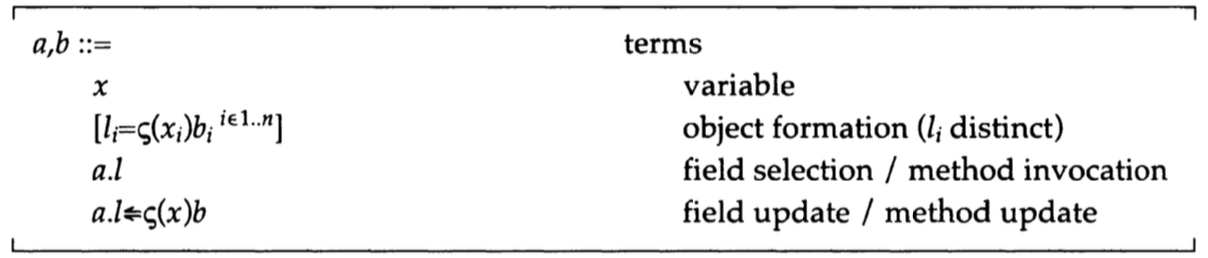
\includegraphics[width=\columnwidth]{syntax}
    \caption{The syntax of untyped Object Calculus as defined by Abadi and Cardelli \cite{ex1}. }
	\label{fig:syntax}
\end{figure}

In Object Calculus, the Methods and Fields of the Objects are not defined individually. Methods and Fields are both defined as a mapping from label to method body in an object \cite{ex11}. Labels are unique in Objects \cite{ex11}, otherwise it can break the mapping in the Object. A Method body without a function is a field \cite{ex1}, and treated as a field of the object. The function body can be construed as an adapted form of Lambda Calculus. 

Objects are defined as a collection (or map from) of labels to methods. The labels are distinct within an object. Methods in an object can be looked up using the labels. 

Method invocation evaluates the body of the method corresponding to the given label in an object, and assigns the result to the method's label and returns it \cite{ex11}. 

Method update is used to add or update the methods of an object \cite{ex1}. It replaces the method corresponding to the given label with the given method, or adds the given method and assigns the given label in the object. 

Objects can be cloned easily in Object Calculus \cite{ex11}. It is required to create multiple objects from an existing template. This can also be represented as a creating objects from classes in class-based object-oriented languages. 

clone(o) produces a new object, with the same labels and the same corresponding methods as Object o \cite{ex11}. 

Inheritance can be demonstrated by cloning an existing object. This is more akin to dynamic inheritance in object-based languages than the class-based inheritance in class-based languages \cite{ex11}. The methods of the cloned object can be updated with different ones or new methods can be added to it. This represents method overriding and polymorphism in conventional object-oriented languages. 

%-------------------------------------------------------------------------
\section{Implementation}

Based on the rules and syntax specified in the previous section we can now implement an Haskell interpreter for untyped imperative Object Calculus. First, we define the data types and then the functions to evaluate method invocation, method update and object cloning. 

\subsection{Object Calculus}
The Object Calculus is defined as a simple data structures in Haskell: 

\begin{lstlisting}
-- Object Calculus Term
data Term =
    Var String
  | Obj Object
  | MetInv String
  | MetUpd String Method
  deriving (Show, Eq)
\end{lstlisting}

We shall break the syntax down and specify what each of them correspond to in the Object Calculus specified by Abadi and Cardelli \cite{ex11}: 

\begin{lstlisting}
Var String
\end{lstlisting}
This refers to the local variable definitions in Object Calculus. Since Haskell is a typed language, we specified it as a String. However, in untyped imperative Object Calculus, it can be of any type. 

\begin{lstlisting}
type Object = (Map String Method)
Obj Object
\end{lstlisting}
This refers to an object in Object Calculus. In Haskell, we defined an Object as a Map (Haskell's Data.Map) between labels(of type String) and Methods. Methods are defined as a separate data type in Haskell. 

\begin{lstlisting}
MetInv String
\end{lstlisting}
This corresponds to Method Invocation of Object Calculus. When evaluated, the Method corresponding to the given label (String) is evaluated. If the Method body is a field and  not a function body then the evaluation simply returns the same field. If the Method body is a function, then it is evaluated in a manner similar to Lambda Calculus and the result is assigned to the same label in the object. 

\begin{lstlisting}
MetUpd String Method
\end{lstlisting}
This corresponds to Method Update of Object Calculus. When evaluated, the Method corresponding to the given label (String) is replaced by the given method. If there is nothing corresponding to the given label, then the given Method is added to the Object as a new Method. As mentioned before, Methods can be Fields or Function Bodies \cite{ex1}. 

\subsection{Object Method and Body}
The Method is another data type defined to be either a field, or a Function Body. 
\begin{lstlisting}
data Method =
    VarM Int
  | Fun Body
  | FunM (Maybe Body)
  deriving (Show, Eq)
\end{lstlisting}
The Method can either be a Field or a Function Body. A Field in this case is defined to be an Integer. However, it can be of any other type as well. The Function Body is defined similar to Lambda Calculus.  

\subsection{Method Invocation}
Method Invocation is defined as a function that evaluates invokes a Method in an Object. It is used by when evaluating the Object Calculus. The label is looked up in the given Object, and the method is evaluated. The function body is evaluated in a manner similar to Lambda Calculus. 
\begin{lstlisting}
-- Method Invocation
methodInvocation :: Object -> String -> Object
methodInvocation obj label = resultantObj where
  m = (lookup label obj)
  m' = evalMethod m
  f m2 = if (m2 == m') then Just m' else Nothing
  resultantObj = Map.update f label obj
  
-- Evaluate a Method
evalMethod :: Method -> Method
evalMethod (VarM number) = VarM number
evalMethod (Fun body) = FunM (evalBody body)
\end{lstlisting}

\subsection{Method Update}
Method Update is simple, and is defined as a function that updates the method corresponding to the given label in an Object. Like Method Invocation, this is also used to evaluate the Object Calculus. The label is looked up in the given Object, and the method is replaced and the modified Object is returned. 
\begin{lstlisting}
-- Update Method with given Method
methodUpdate :: Object -> String -> Method -> Object
methodUpdate obj label m = resultantObj where
  f m' = if (m' == m) then Just m else Nothing
  resultantObj = Map.update f label obj
\end{lstlisting}

\subsection{Object Cloning}
This is the simplest one of the functions. It simply returns the same object, as a copy. Method update can be applied on the copy to obtain a derived object, this represents object-based inheritance in many object-based languages. 
\begin{lstlisting}
-- Clone an object
objClone :: Object -> Object
objClone obj = obj
\end{lstlisting}

%-------------------------------------------------------------------------
\section{Conclusion}

The Haskell interpreter for Object Calculus can be used to gain a better understanding of how Object-oriented languages are represented using Object Calculi. As we mentioned in a previous section, there are other approaches to modeling object-oriented languages. However, we chose to build upon Abadi and Cardelli's Object Calculus because we feel it is a more generic representation of object-oriented languages and hence can be used to model any type of object oriented language \cite{ex1}. 

Mapping Object Calculus devised for representing Object-Oriented Languages in a Functional Language like Haskell has been quite difficult. Untyped Imperative Object Calculus is the more generic and minimal form of Object Calculus. But as Haskell is a typed functional language with lazy evaluation, there is often a mismatch between the implementation, and the given typing rules, semantics and the Object Calculus syntax. Unfortunately, the current implementation of the interpreter does not fully parse the more advanced expressions in Object Calculus. But it is able to parse and evaluate the untyped imperative Object Calculi of the previous sections. 

In the future, this interpreter can be extended to support Typed Object Calculus as well \cite{ex5}. A Type system for the Object Calculus has already been devised by Abadi and Cardelli \cite{ex11}. However, whether it is feasible to do so in Haskell remains to be seen. 

%-------------------------------------------------------------------------

\bibliographystyle{latex8}
\bibliography{latex8}

\end{document}
